\documentclass[archE1,portrait]{baposter}

% Tamaño del póster: 841mm x 1189mm (A0)
\usepackage[utf8]{inputenc}
\usepackage[spanish]{babel}
\usepackage[font=small,labelfont=bf]{caption}
\usepackage{booktabs}
\usepackage{amsmath}
\usepackage{physics}
\usepackage{graphicx}
\usepackage[urlcolor = blue]{hyperref}

\graphicspath{{figures/}}

% --- Definición de colores ---
\definecolor{bordercol}{RGB}{5,2,82}      % Color del borde de las cajas
\definecolor{headercol1}{RGB}{30,64,120}  % Color de fondo para el encabezado (azul oscuro)
\definecolor{headercol2}{RGB}{30,64,120}  % Color de fondo para el encabezado (lado derecho)
\definecolor{headerfontcol}{RGB}{255,255,255} % Color del texto del encabezado (blanco)
\definecolor{boxcolor}{RGB}{245,245,255}  % Color de fondo del contenido (azul muy claro)

\begin{document}

\background{}

\begin{poster}{
    grid=false,
    borderColor=bordercol,
    headerColorOne=headercol1,
    headerColorTwo=headercol1,
    headerFontColor=headerfontcol,
    boxColorOne=boxcolor,
    headershape=roundedright,
    headerfont=\Normal\sf\bf,
    textborder=rectangle,
    background=user,
    headerborder=open,
    boxshade=plain
}
%
%----------------------------------------------------------------------------------------
%   TÍTULO Y AUTORES
%----------------------------------------------------------------------------------------
%
%----------------------------------------------------------------------------------------
%   INTRODUCCIÓN Y MOTIVACIÓN
%----------------------------------------------------------------------------------------

\headerbox{Introducción y Motivación}{name=intro,column=0,row=0,span=3}{
La enseñanza de la mecánica cuántica suele centrarse en resolver analíticamente un conjunto limitado de sistemas ideales. Sin embargo, la física moderna se apoya cada vez más en el cómputo científico para estudiar sistemas complejos y no triviales.
En este proyecto se desarrollaron implementaciones en Python de métodos fundamentales —el algoritmo de Numerov y el método de Hartree–Fock— con el doble propósito de profundizar en su estructura teórica y ofrecer una herramienta accesible para la exploración computacional de sistemas cuánticos.

}

% ----------------------------------
%  RESULTADOS Y APLICACIONES
% ----------------------------------

\headerbox{Numerov}{name=numerov,column=0,below=intro,span=2}{

El método de Numerov permite integrar ecuaciones diferenciales de segundo orden como la ecuación de Schrödinger adimensional:

\begin{equation}
\label{eq:1}
\pdv[2]{\Psi}{\xi} = -2\qty(\epsilon - \frac{\xi}{2})\Psi
\end{equation}

Discretizando el dominio y utilizando la recurrencia:

\begin{equation}
\label{eq:2}
\Psi_{n+1} = 
\frac{(12 - 10 f_n) \Psi_n - f_{n-1} \Psi_{n-1}}{f_{n+1}}
\end{equation}

\begin{itemize}
  \item Utilizamos física para diseñar el algoritmo de integración.
  \item El mismo algoritmo se adapta fácilmente a distintos potenciales (\textit{p.ej.}, oscilador armónico y átomo de hidrógeno).
\end{itemize}

\begin{center}
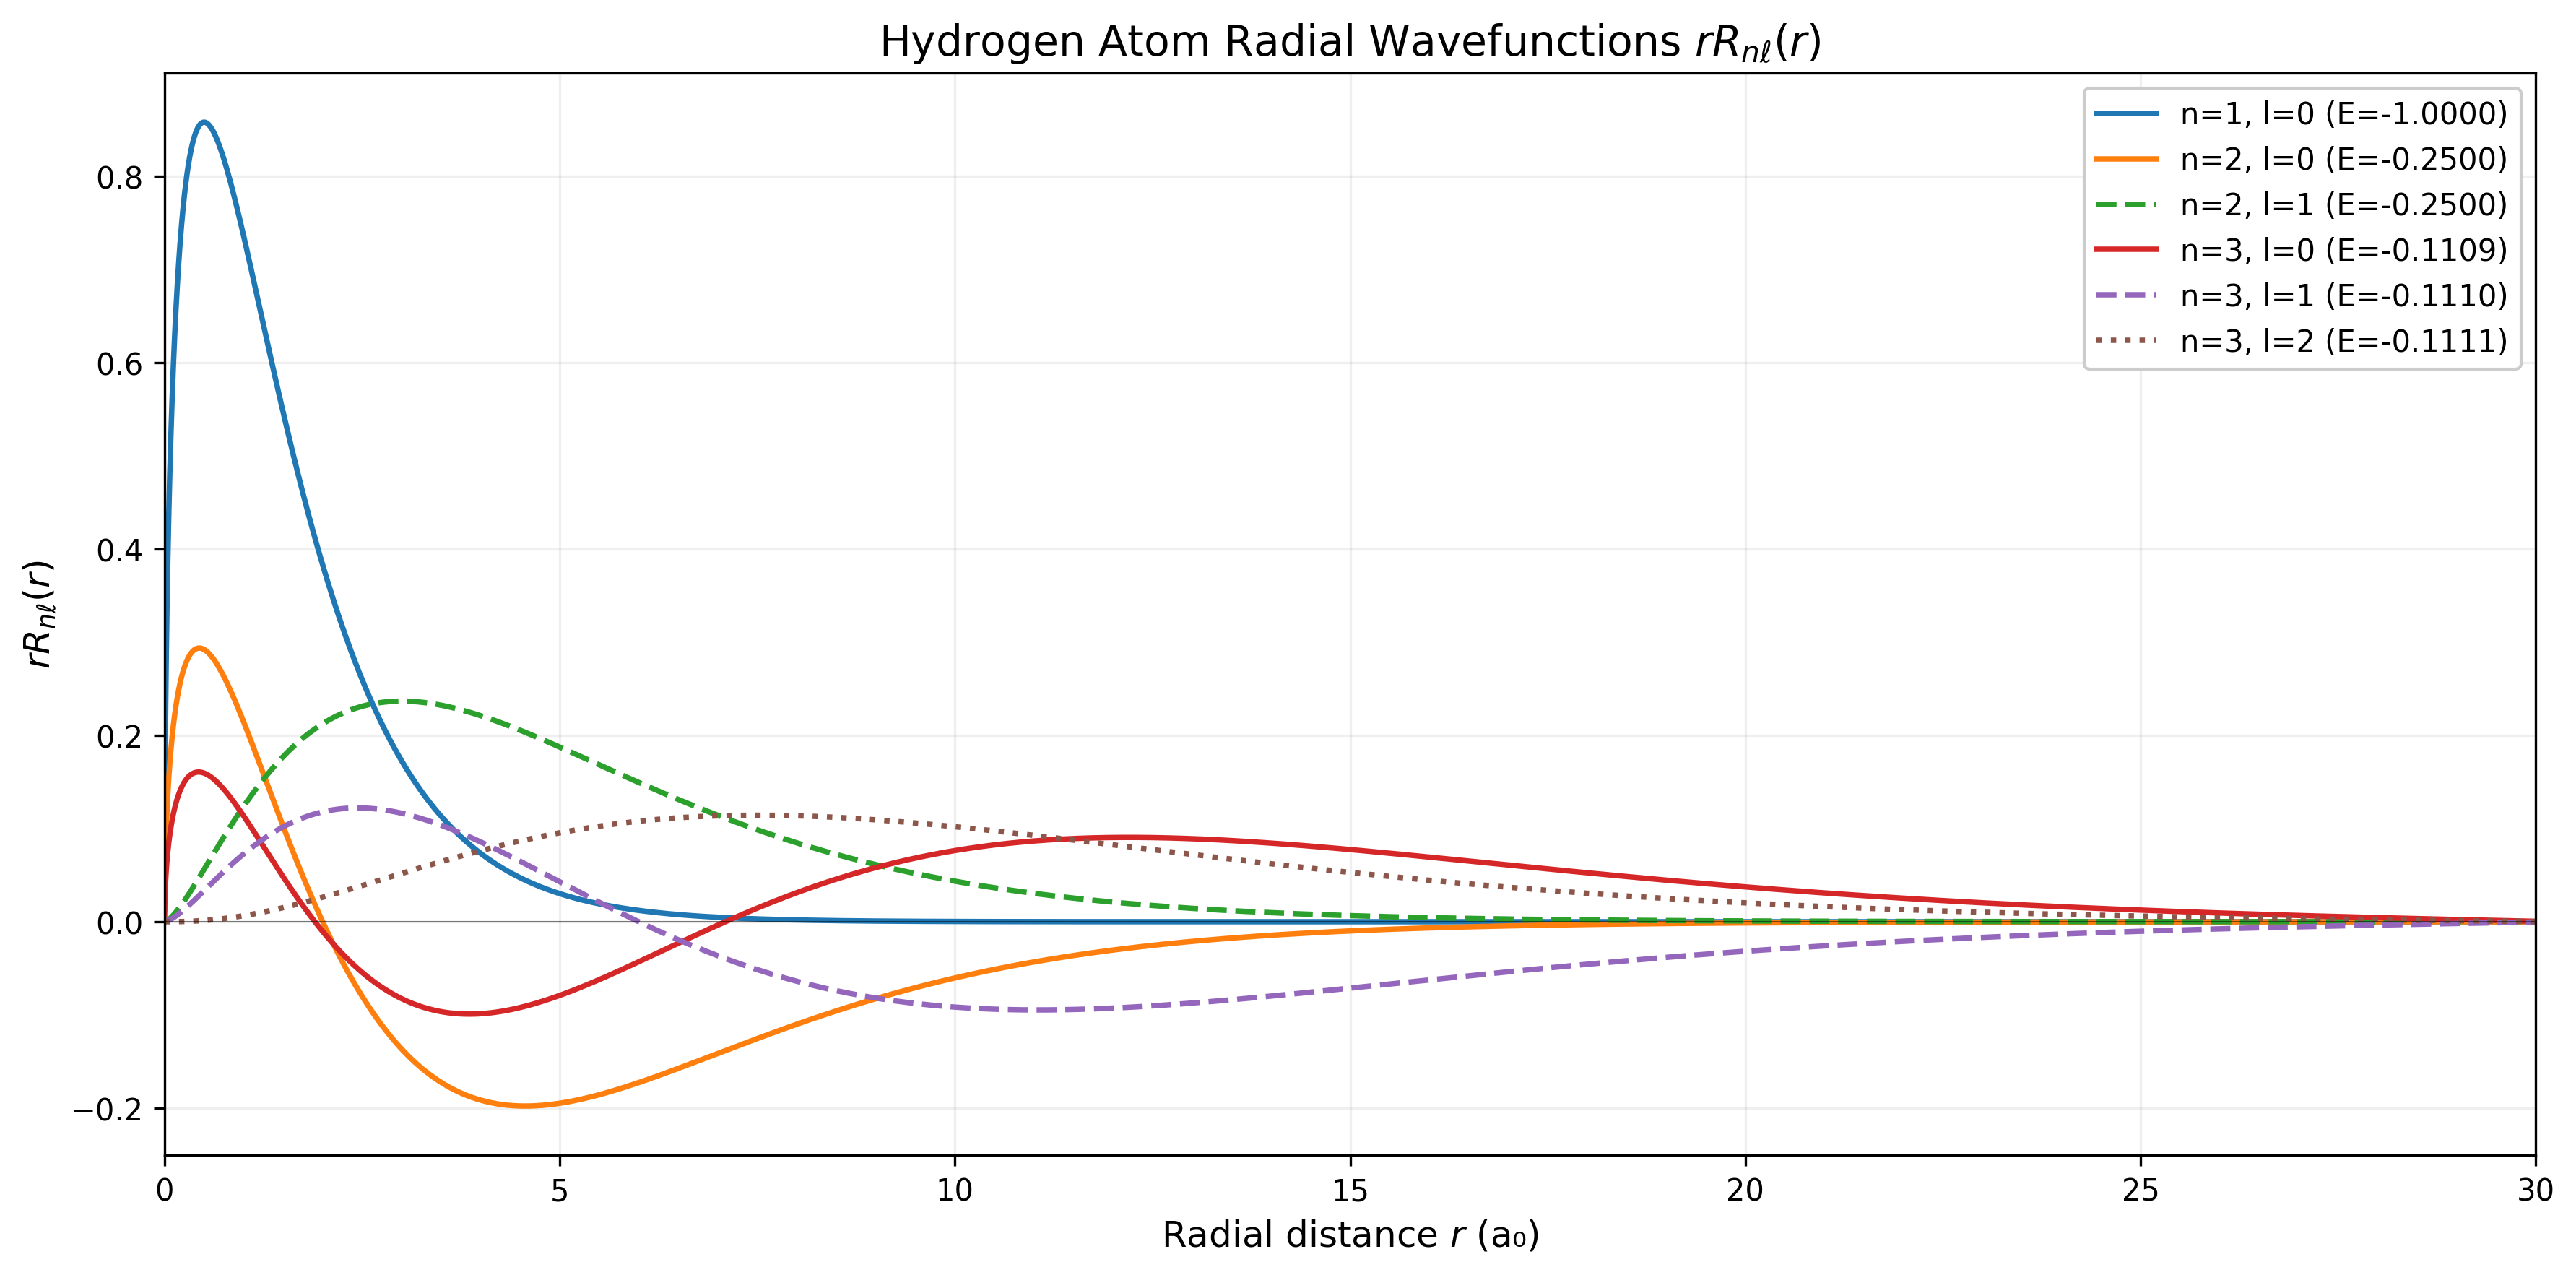
\includegraphics[width=0.9\linewidth]{hydrogen.png}
\captionof{figure}{Funciones de onda radiales obtenidas con Numerov.}
\end{center}
  
}

\headerbox{Método de Hartree–Fock}{name=hf,column=0,below=numerov,span=3}{
El método de Hartree–Fock aproxima el estado fundamental de un sistema de $N$ electrones mediante un determinante de Slater que minimiza la energía total bajo el principio variacional.  

Partiendo de la formulación matricial de Roothaan–Hall:

\[
\mathbf{F}\mathbf{C} = \mathbf{S}\mathbf{C}\boldsymbol{\varepsilon}
\tag{3}
\]

donde $\mathbf{F}$ es la matriz de Fock, $\mathbf{S}$ la de solapamiento, $\mathbf{C}$ los coeficientes moleculares y $\boldsymbol{\varepsilon}$ los valores propios orbitales.

El proceso se resuelve mediante un ciclo de autoconsistencia (SCF):

\textbf{Ciclo SCF (esquema):}
\begin{center}
\begin{tikzpicture}[
  node distance=1.6cm, every node/.style={align=center},
  box/.style={rounded corners, draw=primary, very thick, fill=white, inner sep=6pt},
  >={Stealth[length=6pt]}
]
\node[box] (int) {Integrales \\ $S,\,T,\,V,\,$ERIs};
\node[box, below=of int] (fock) {Construir $\mathbf{F}[\mathbf{P}]$};
\node[box, below=of fock] (diag) {Diagonalizar \\ $\mathbf{F'}\mathbf{C'}=\mathbf{C'}\varepsilon$};
\node[box, below=of diag] (dens) {Actualizar $\mathbf{P}=2\,\mathbf{C}_{\text{occ}}\mathbf{C}_{\text{occ}}^\top$};
\draw[->,thick] (int) -- (fock);
\draw[->,thick] (fock) -- (diag);
\draw[->,thick] (diag) -- (dens);
\draw[->,thick] (dens) to[bend right=50] node[right]{\small hasta converger} (fock);
\end{tikzpicture}
\end{center}

\begin{itemize}
  \item Permite obtener energías y orbitales moleculares a partir del principio variacional.
  \item La densidad electrónica resultante describe la distribución espacial de los electrones.
  \item Sirve como punto de partida para métodos de correlación y teoría del funcional de la densidad (DFT).
\end{itemize}

\begin{center}
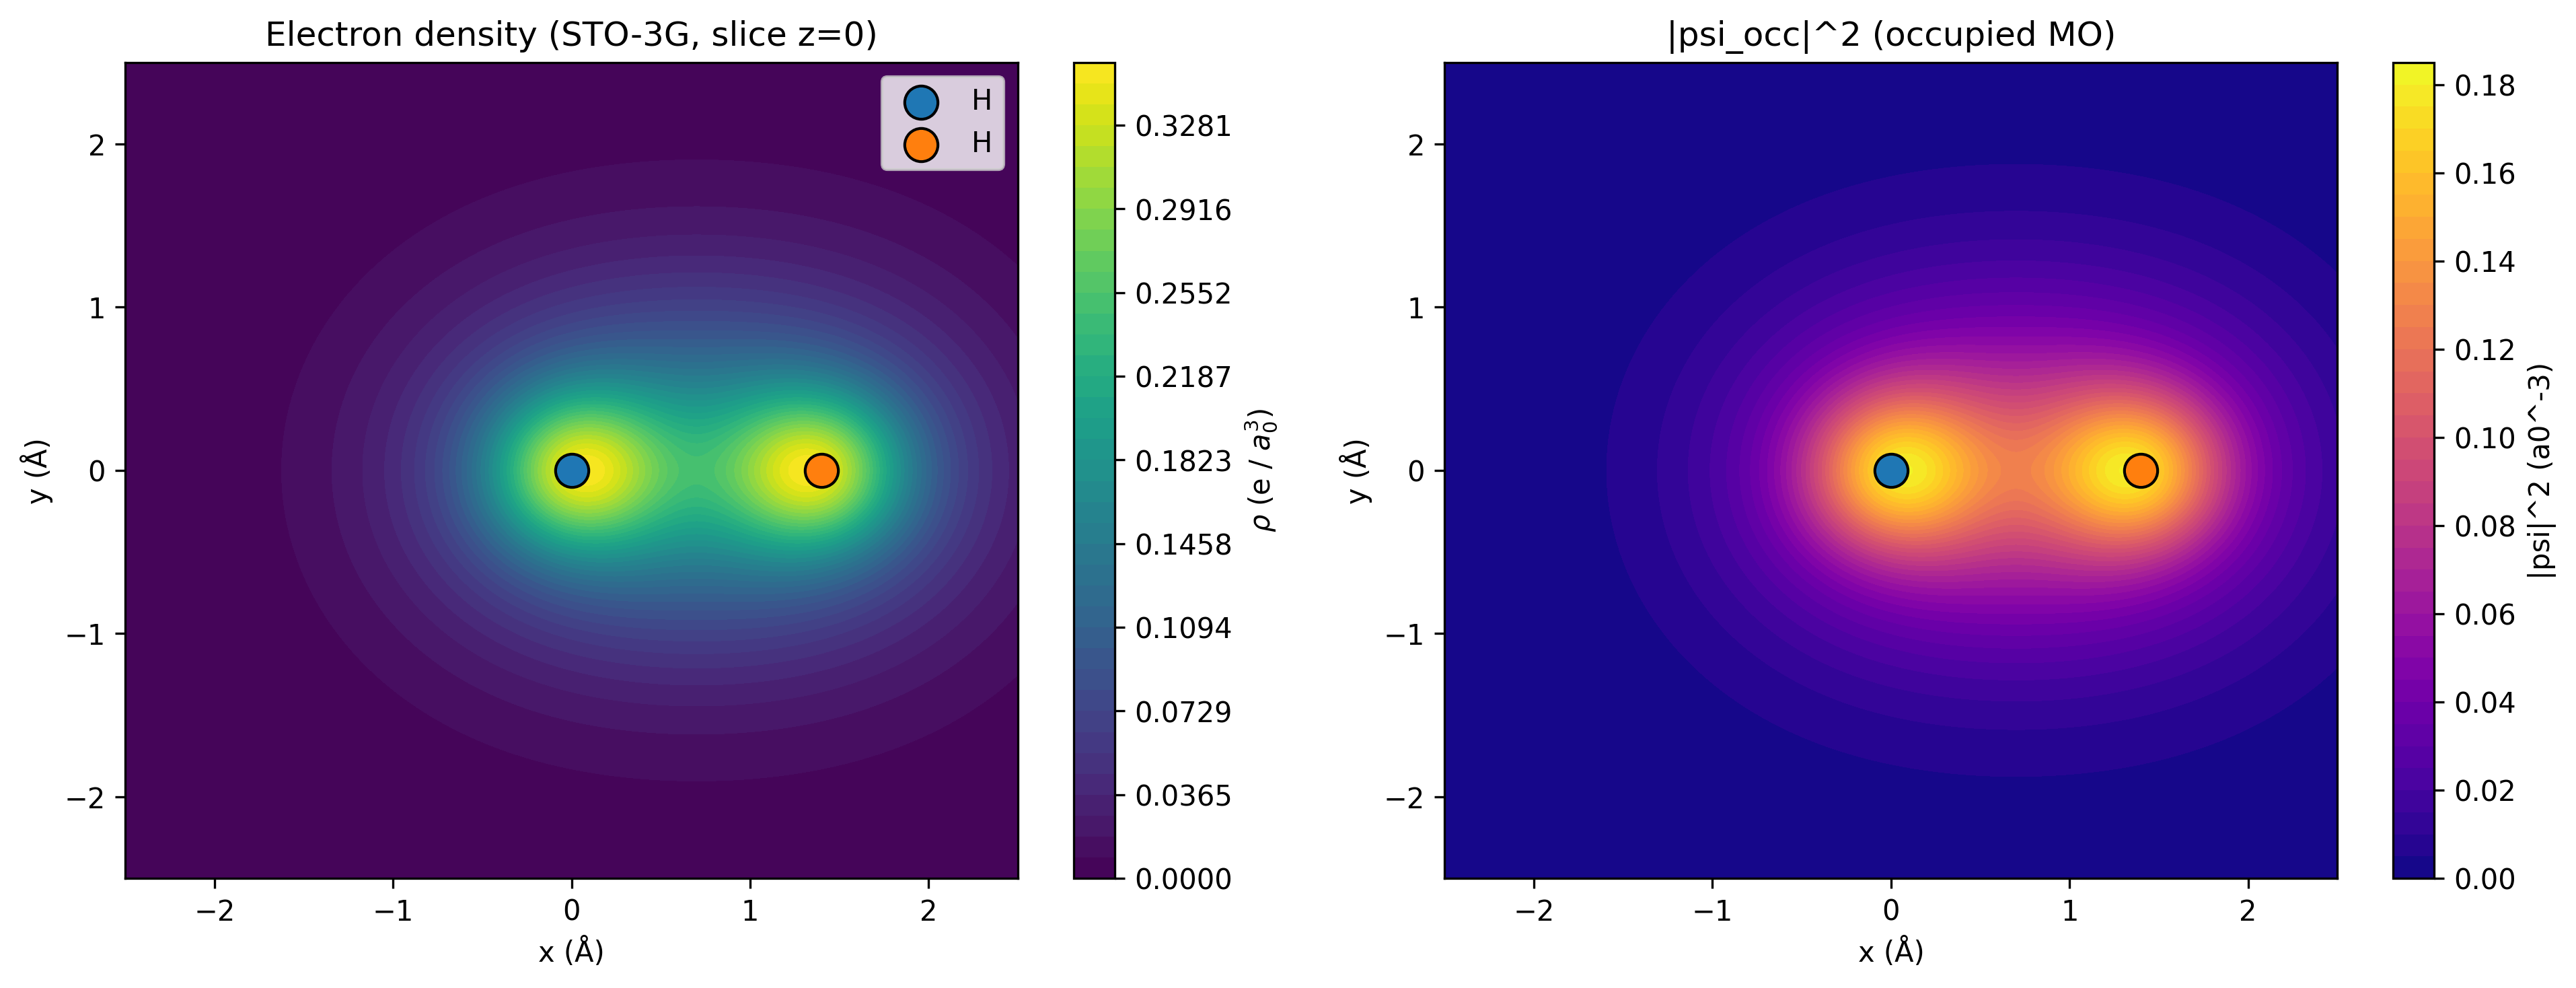
\includegraphics[width=0.9\linewidth]{hf_h2.png}
\captionof{figure}{Densidad electrónica de la molécula de H$_2$ calculada en el nivel Hartree–Fock.}
\end{center}
}

\end{poster}
\end{document}
